\documentclass[xcolor=x11names,compress,professionalfonts]{beamer}

%% General packages %%%%%%%%%%%%%%%%%%%%%%%%%%%%%%%%%%
\usepackage[utf8]{inputenc}
\usepackage{graphicx}
\usepackage{tikz}
\tikzset{% change default arrow tips
    >=latex
}
\usepackage{ifthen}

\usepackage{amsmath}
\usepackage{nicefrac}

\usepackage{color}

% compile child documents using this preamble
\usepackage{subfiles}

% compile child files with separate preambles, and include them in the document
\usepackage{standalone}

%%%%%%%%%%%%%%%%%%%%%%%%%%%%%%%%%%%%%%%%%%%%%%%%%%%%%%

\makeatletter
\setbeamertemplate{footline}
{
    \leavevmode%
    \hbox{%
        \begin{beamercolorbox}[wd=.333333\paperwidth,ht=2.25ex,dp=1ex,center]{author in head/foot}%
            \usebeamerfont{author in head/foot}\insertshortauthor
        \end{beamercolorbox}%
                \begin{beamercolorbox}[wd=.333333\paperwidth,ht=2.25ex,dp=1ex,center]{title in head/foot}%
            \usebeamerfont{title in head/foot}\insertshorttitle
        \end{beamercolorbox}%
        \begin{beamercolorbox}[wd=.333333\paperwidth,ht=2.25ex,dp=1ex,right]{date in head/foot}%
            \usebeamerfont{date in head/foot}\insertshortdate{}\hspace*{2em}
            \insertframenumber{} / \inserttotalframenumber\hspace*{2ex} 
        \end{beamercolorbox}}%
        \vskip0pt%
    }
    \makeatother


%% Beamer Layout %%%%%%%%%%%%%%%%%%%%%%%%%%%%%%%%%%
\useoutertheme[subsection=false,shadow]{miniframes}
\useinnertheme{rectangles}

\setbeamertemplate{navigation symbols}{}%remove navigation symbols

\author{Nicolas Macé}

\newcommand{\btVFill}{\vskip0pt plus 1filll}%place an element at the bottom of the page

\usepackage{libertine}
\usepackage[T1]{fontenc}

\setbeamerfont{title like}{shape=\scshape}
\setbeamerfont{frametitle}{shape=\scshape}

\setbeamercolor*{lower separation line head}{bg=DeepSkyBlue4} 
\setbeamercolor*{normal text}{fg=black,bg=white} 
\setbeamercolor*{alerted text}{fg=red} 
\setbeamercolor*{example text}{fg=black} 
\setbeamercolor*{structure}{fg=black} 
 
\setbeamercolor*{palette tertiary}{fg=black,bg=black!10} 
\setbeamercolor*{palette quaternary}{fg=black,bg=black!10} 

\renewcommand{\(}{\begin{columns}}
\renewcommand{\)}{\end{columns}}
\newcommand{\<}[1]{\begin{column}{#1}}
\renewcommand{\>}{\end{column}}

\definecolor{BostonBlue}{HTML}{00688B}
\definecolor{Complementary}{HTML}{8B2300}

\renewcommand{\ss}[1]{\scriptsize{\text{#1}}}
%%%%%%%%%%%%%%%%%%%%%%%%%%%%%%%%%%%%%%%%%%%%%%%%%%

\usepackage{braket}
% compile child documents using this preamble
\usepackage{subfiles}

%%%My Math

\newcommand{\pd}[2]{\frac{\displaystyle \partial #1}{\displaystyle\partial #2}} % for partial derivatives
\renewcommand{\d}[1]{\mathrm{d}#1}

\begin{document}

\begin{frame}
\title{{\fontsize{14}{60}\selectfont Exact results on electronic wavefunctions of 2D quasicrystals}}

\author{Nicolas Macé, Anuradha Jagannathan, Frédéric Piéchon}

\institute % (optional)
{
  Laboratoire de Physique des Solides\\
  Université Paris-Saclay
}

\date{September 20, 2016}

\titlepage

\btVFill
\begin{columns}
\begin{column}{2cm}
~\\
~\\
~\\
~\\
\raggedright

\includegraphics[scale=.15]{img/LogoUPSUD.png}
\end{column}
\begin{column}{6cm}
\centering
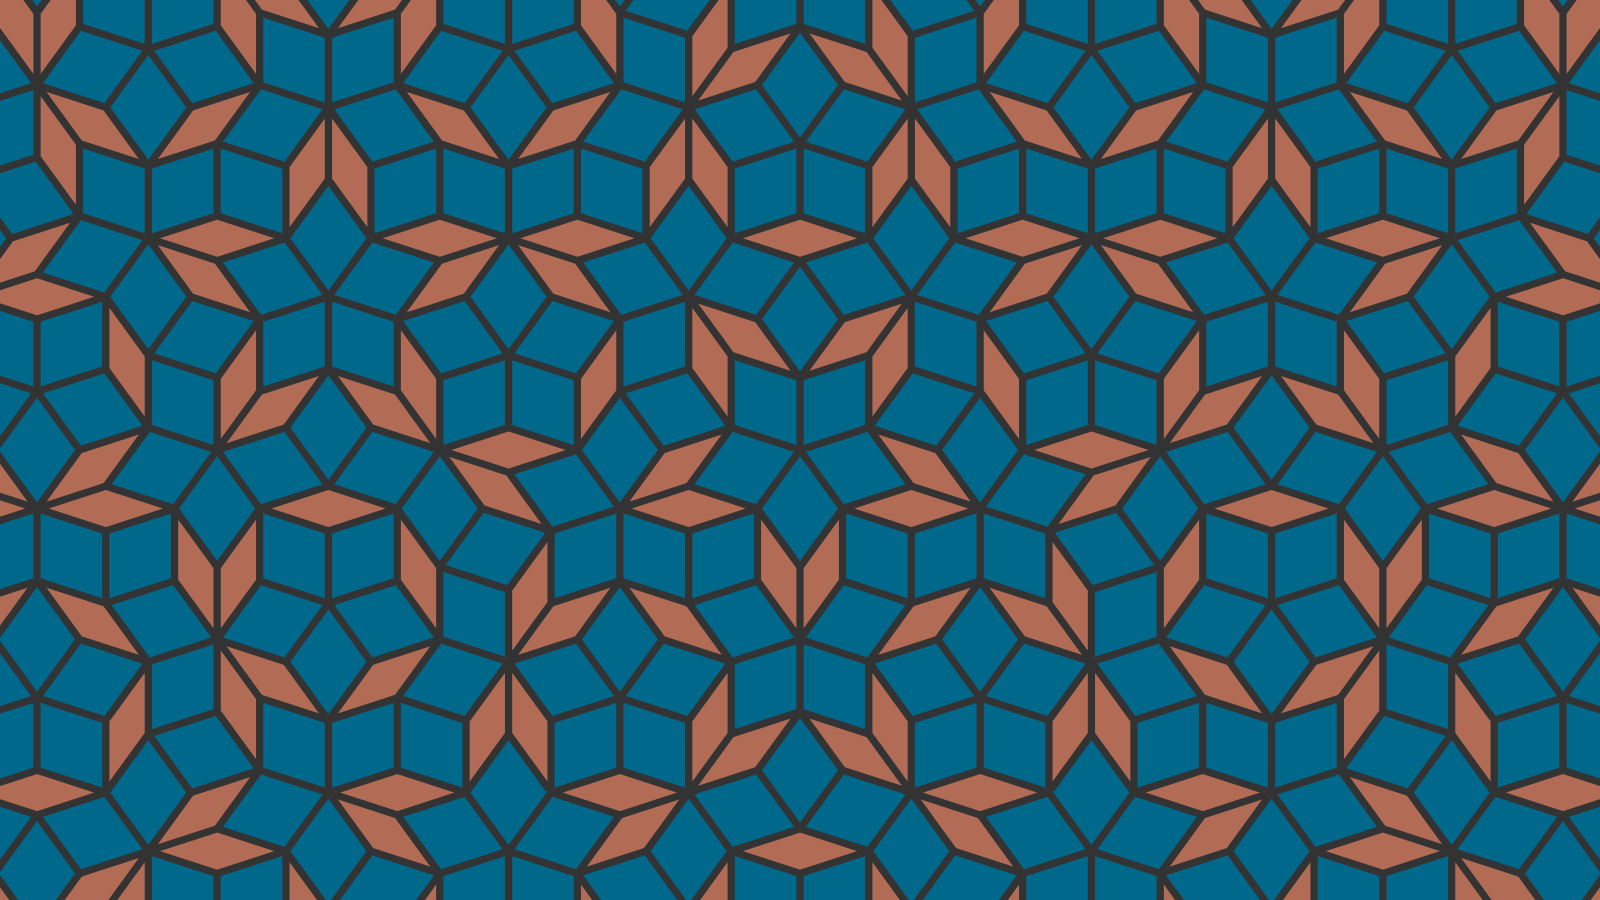
\includegraphics[width=.7\textwidth]{img/cover.png}
\end{column}
\begin{column}{2cm}
~\\
~\\
~\\
~\\
\raggedleft

\includegraphics[scale=.15]{img/logo-lps.jpg}
\end{column}
\end{columns}
\end{frame}

\begin{frame}{Electronic properties of quasicrystals}
We can we do to access the electronic properties of quasicrystals?
\begin{itemize}
	\item Experiments
	\begin{itemize}
		\item Measure of physical properties: conductivity, ???
	\end{itemize}
	\item ``Realistic'' simulations
	\begin{itemize}
		\item Direct access to the electronic states 
	\end{itemize}
	\item Toy models
	\begin{itemize}
		\item More managable (sometimes exactly solvable) $\rightarrow$ easier to see the consequences of quasiperiodicity
		\item Simple states can be seen as ``building block'' for more realistic ones (like Bloch's states for periodic materials)
	\end{itemize}
\end{itemize}

\end{frame}

\begin{frame}
\frametitle{Toy models of quasicrystals}
We want to model:
\begin{itemize}
	\item a single electron (ie we do not consider interactions)
	\item on a quasiperiodic tiling, in 1D or in 2D
	\item in the simplest possible way : tight-binding model with nearest neighbors hoppings only
\end{itemize}
\[
	i \frac{\partial \phi_m}{\partial t}(t) = \sum_{n \in V(m)} t_{m,n} \phi_n(t) ~\text{with}~ |\phi_m(t)|^2= \text{Prob}\left( \text{on atom $m$ at time $t$} \right)
\]

[Picture of the hoppings on a tiling]

We solve for the stationary states (or eigenstates):
\[
	E \psi_m = \sum_{n \in V(m)} t_{m,n} \psi_n
\]
Challenge: find a proper description of these eigenstates... 
\end{frame}

\begin{frame}
\frametitle{What is known: periodic and disordered models}
\begin{itemize}
	\item Eigenstates on periodic materials: 
	\begin{itemize}
		\item Plane waves 
		\item \textbf{constant} amplitude $\rightarrow$ \textbf{extended states}
	\end{itemize}
	\subfile{img/periodic_chain.tex}
	\item Eigenstates on disordered materials: 
	\begin{itemize}
		\item Evanescent waves
		\item  \textbf{exponentially decreasing} amplitude $\rightarrow$ \textbf{localized states}
	\end{itemize}
	\subfile{img/disordered_chain.tex}
\end{itemize}
\textbf{What about quasiperiodic materials?}

\textcolor{Complementary}{We will see on examples their electrons are somewhat \textbf{in between}: the wavefunctions have local power law decay, they are \textbf{critical}}
\end{frame}

\begin{frame}
\frametitle{Outline}
\tableofcontents[hideallsubsections]
\end{frame}

\section{Quasiperiodic chains}
%Each section needs a subsection for the small points on top to show up
\subsection{Dummy}

\begin{frame}{Cut and project chains}
		The geometrical model:
		
		{\centering
		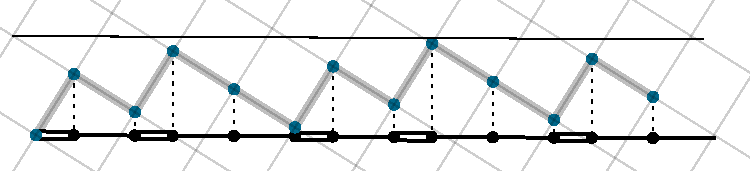
\includegraphics[scale=0.8]{img/cut_and_project_Fibonacci.pdf}
		
		}
		
		The corresponding chain of atoms:
		
		{\centering
		\subfile{img/fibo_chain.tex}
		
		}
The Schrödinger equation for the eigenstate of energy $E$:
\[
	 t_{m-1,m} \psi_{m-1} + t_{m,m+1}\psi_{m+1} = E \psi_{m}
\]
\[
	t_{m-1,m} = t_s \text{~or~} t_w \text{~and we set $t_s = 1$, $t_w = \rho$}
\]
What can be say about the spectrum/eigenstates of this model?
\end{frame}

\begin{frame}{Spectrum/eigenstates of cut and project chains}
\begin{itemize}
	\item The spectrum is scale invariant (or multifractal)
	
{\centering
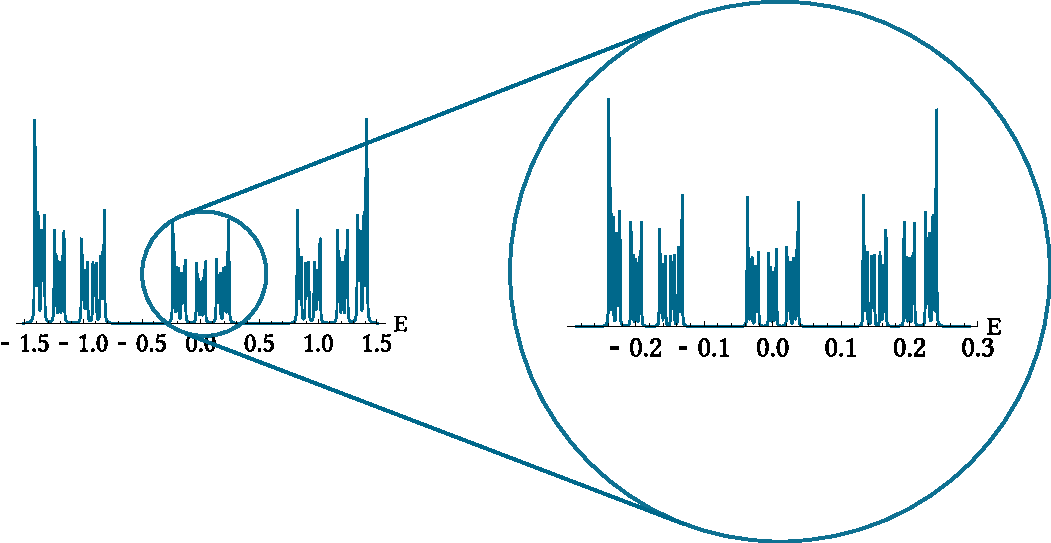
\includegraphics[scale=.5]{img/ldos.pdf}

}
	\item The eigenstates are generically critical (all of them are for the Fibonacci chain [reference])
\end{itemize}
What is the structure of these critical states?
\end{frame}

\begin{frame}{A special case: the eigenstate at zero energy}
\begin{itemize}
	\item Schrödinger equation for the $E=0$ state:
	\[
	t_{m-1,m} \psi_{m-1} + t_{m,m+1}\psi_{m+1} = 0
	\]
	\item If we know the wavefunction on one site we know it on the next
	\begin{columns}
	\<{6cm}
	\[
	\psi_{m+1} = -\frac{t_{m-1,m}}{t_{m,m+1}} \psi_{m-1}
	\]
	\>
	\<{5cm}
	\subfile{img/hop_E0.tex}
	\>
	\end{columns}
	\item Introduce $A_{m-1,m+1}$, the \textbf{arrow} from $m-1$ to $m+1$:
	\begin{columns}
	\<{5cm}
	\centering
	 \subfile{img/hop_right.tex}
	 \>
	 \<{5cm}
	 Remember that $\rho = t_s/t_w$.
	 
	Then, $\boxed{\psi_{m+1} =- \rho^{A_{m-1,m+1}} \psi_{m-1}}$
	 \>
	 \end{columns}
\end{itemize}
\end{frame}

\begin{frame}{The field of arrows and the field of heights}
From $\psi_{m+1} =- \rho^{A_{m-1,m+1}} \psi_{m-1}$ we deduce that
\[
	\psi_{2m} = (-1)^{m} \psi_0 \rho^{h(m)}
\]
Where $h$ is \textbf{the field of heights}, the integral of the field of arrows:
\[
	h(m) = \sum_{n=0}^m A_{n, n+2}
\]



\end{frame}

\begin{frame}{Back to the special cases, with arrows!}
\begin{itemize}
	\item Periodic chain: no arrows $\rightarrow$ extended
	\item Disordered chain: random arrows $\rightarrow$ $\langle h \rangle = 0$: localized
\end{itemize}
\end{frame}

\begin{frame}{Fibo and the inflation}
\begin{itemize}
	\item Inflation rule $\phi: A \to AB,\dots$
	\item Concepts of atoms and molecules, spectrum seen as broadening of atomic ($E=0$) and molecular ($E = \pm 1$) levels.
	\item Atomic inflation ($\phi^3$) should be relevant since we expect the $E=0$ wf to have have mainly weight on the atomic sites
	\item Indeed yes: $\phi^3$ is an inflation rule for the arrows: $\phi^3: R \to \dots, L \to \dots$
\end{itemize}
\end{frame}

\begin{frame}{The Fibo arrows and the Fibo wf}
\begin{itemize}
	\item On old sites height is constant $\rightarrow$ cannot be localized
	\item On new sites height increases at most linearly $\rightarrow$ $\log L$ growth, local power law behavior
	\item Rigorously: $IPR$ computed analytically from the arrow statistics $\rightarrow$ critical wf.
\end{itemize}
\end{frame}

\begin{frame}{Summing up what happens in 1D}
\begin{itemize}
	\item max height $\sim \log L$, typical height $\sim \sqrt{\log L}$
	\item Arrow is a quasiperiodic function
	\item Its integral, the height, is not
	\item As a result, the wf is critical: it behaves locally as a power law
	\item We will find again all these features in 2D
\end{itemize}
\end{frame}

\begin{frame}{Cut and project 1D models are special!}
\begin{itemize}
	\item B3 substitution: a two letters, deterministic chain, that is non-Pisot $\rightarrow$ cannot be built by cut and project.
	\item Height resembles a random walk, and typical height $\sim \sqrt{L}$
	\item $\rightarrow$ wf localized 
\end{itemize}
\end{frame}

\section{2D case}
\subsection{Dummy}

\begin{frame}{Construction of the model: Ammann-Beenker and Penrose}
\begin{columns}
\begin{column}{5cm}
{\centering
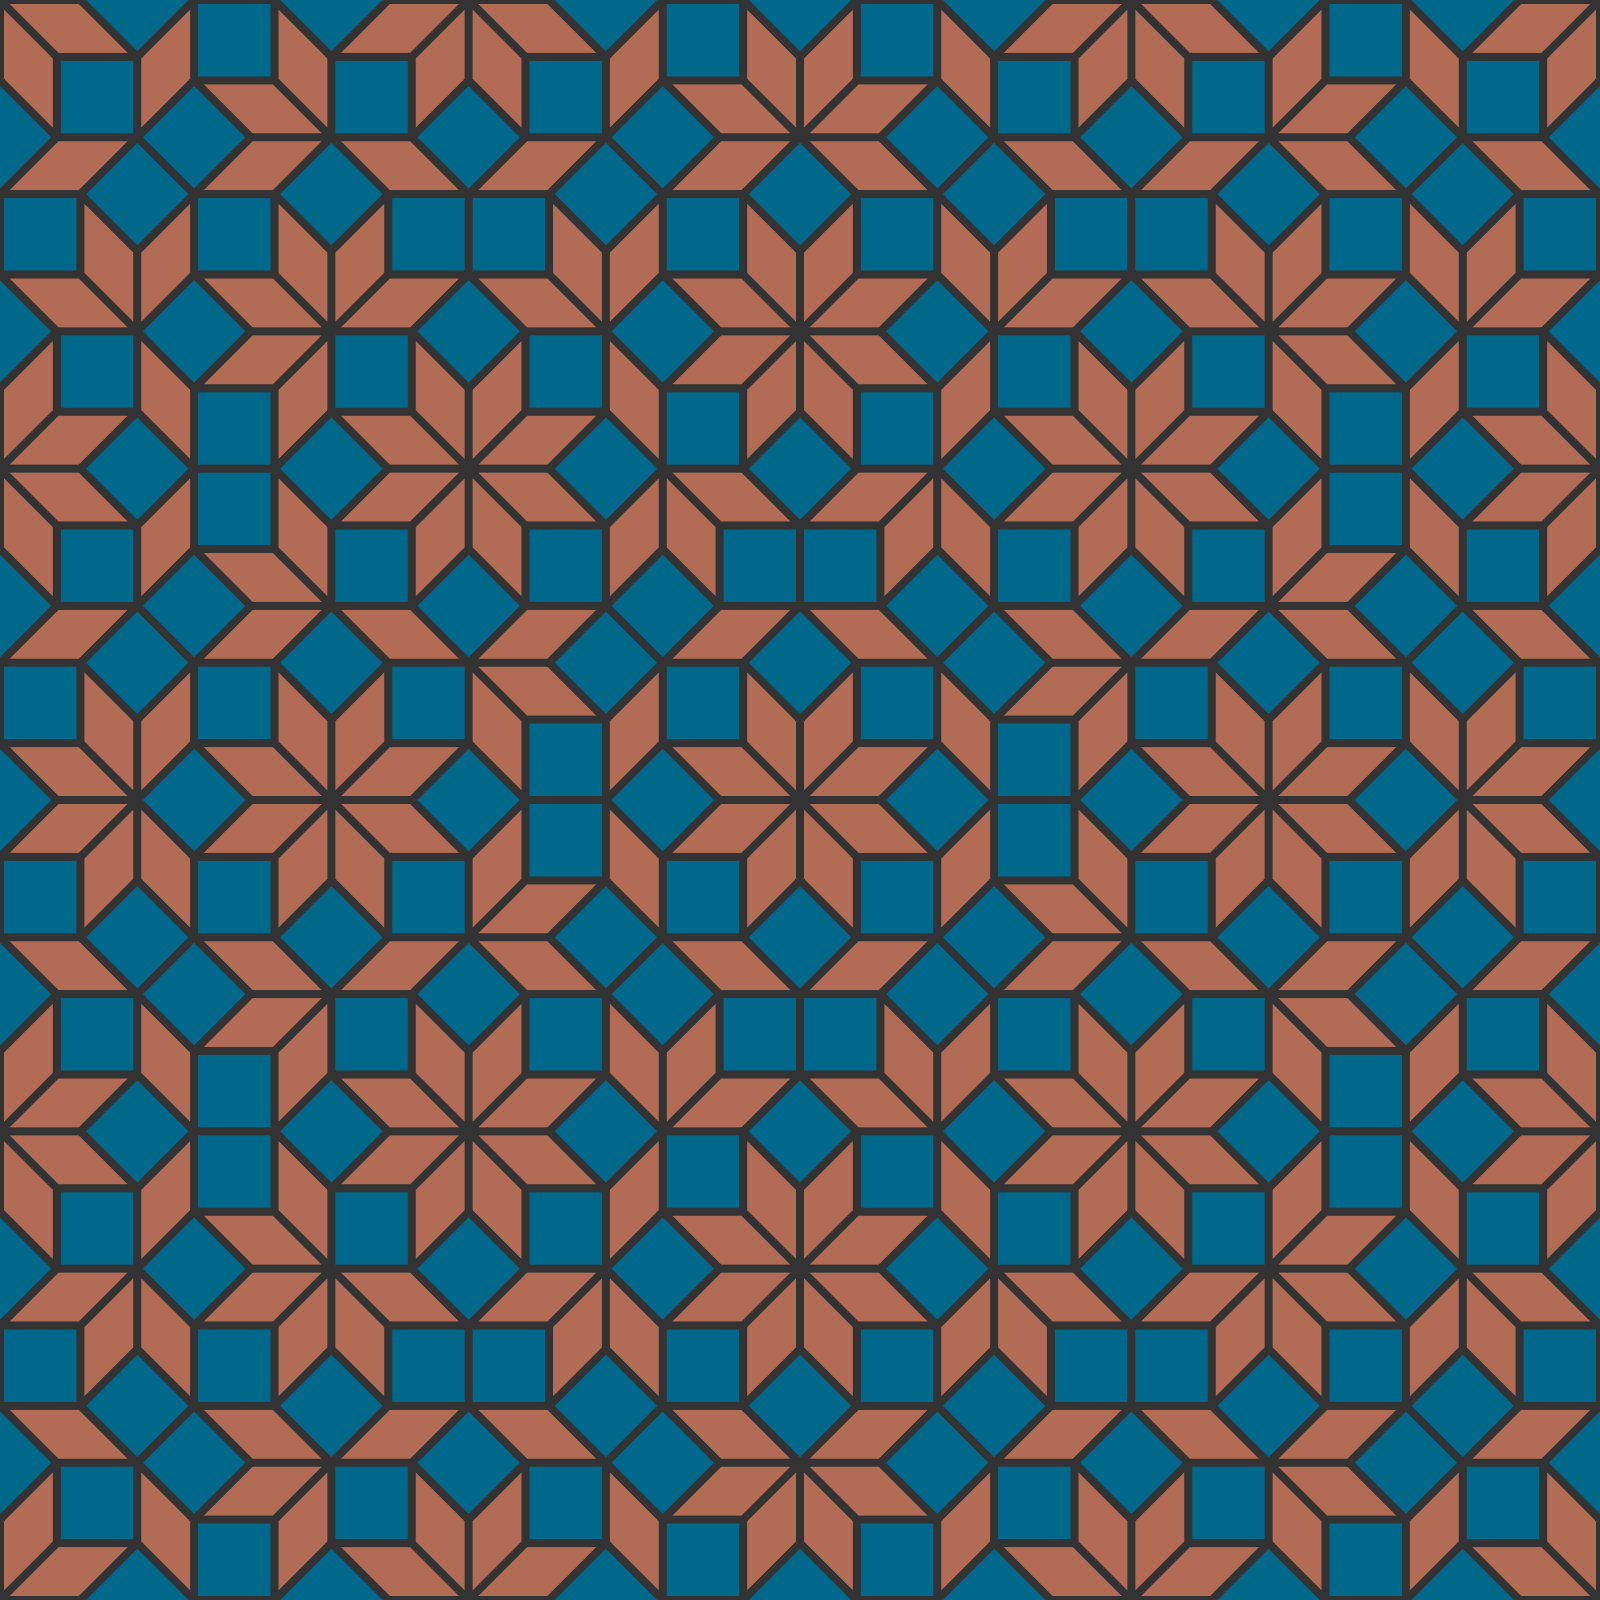
\includegraphics[scale=.1]{img/ammann-beenker.png}

}
\end{column}
\begin{column}{5cm}
\[
	-\sum_{n \in V(m)} \psi_n = E \psi_m
\]
No parameters: the quasiperiodic features are encoded in the adjacency of the vertices.
\end{column}
\end{columns}
\end{frame}

\begin{frame}{What is known}
\begin{itemize}
	\item Spectrum is more regular: only a few gaps, no apparent fractal structure
	\item $E = 0$ wfs are localized: too bad!
	\item The other wf are critical (numerical result)
\end{itemize}
$\rightarrow$ can we introduce a field of arrows to describe some of these critical wfs?
\end{frame}

\begin{frame}{The ground state}
\begin{itemize}
	\item Sutherland's idea: introduce local potentials to make the construction of the grounstate simpler.
	\item Sutherland's groundstates on Penrose and AB tilings is constructed via the introduction of a field of arrows, exactly like the 1D ones
\end{itemize}
$\rightarrow$ what are the properties of this field of arrows?
\end{frame}

\begin{frame}{Inflation and the field of arrows}
Here we focus on the AB example, but everything works the same for Penrose.
\begin{itemize}
	\item Arrows $\leftrightarrow$ matching rules for the tiles 
	\item Matching rules are enforced by the inflation rules $\rightarrow$ we should be able to study the properties of the arrows via the inflation (just like in 1D)
	\item From the inflation rules, we deduce the maximal height $\sim \log L$
	\item Statistics of the heights $P_\mu^{l}(h)$ obeys a diffusion-like equation where $l$ plays the role of time and $h$ the role of space
	\item $\rightarrow$ typical height is $\sim \sqrt{\log L}$
\end{itemize}
So we understand everything about Stutherland's wavefunction, but the model has been built for this wavefunction to exist. 
Can we use this field of arrows to describe wavefunctions on more realistic models?
Yes: Pavel.
\end{frame}

\begin{frame}{Characterization of the groundstate wavefunction}
\begin{itemize}
	\item We go back to the model with no local potentials. 
	\item From the plot of the groundstate: we see a complicated local structure (role of the local environment) and the phason line (role of the arrow field)
	\item Indeed, the wf decomposes into a local part and an arrow part (this was guessed from involved algebraic arguments).
	\item Computation of the IPR scaling and the multifractal exponents: the local part doesn't play any role $\rightarrow$ exponents only sensitive to the arrow part, ie to the quasiperiodicity!
	\item Remains valid for a larger class of models $H = \sum_{\langle i, j \rangle} \ket{i} \bra{j} + V_i \ket{i} \bra{i} $
\end{itemize}
\end{frame}

\begin{frame}{Conclusion}
\begin{itemize}
	\item Non-interacting eigenstates on quasicrystals are generically critical: here we were able to understand it for some specific states, both in 1D and 2D.
	\item On our examples, wavefunction construction involves a geometrical quasiperiodic function, the field of arrows.
	\item Its integral, the height function, has logarithmic growth,
	\item As a result, the wavefunction is critical: it has a local power law behavior.
\end{itemize}
Perspectives:
\begin{itemize}
	\item What happens for the grounstate of other quasicrystals, like the dodecagonal ones?
	\item For Penrose and AB, the arrow field cannot be used to describe other states. What extra ingredients are required?
\end{itemize}
\end{frame}

\begin{frame}{More perpsectives!}
\begin{itemize}
	\item A plot of the state just below the gap, with its quasiperiodic array of lines of zeros, that remain to be understood!
\end{itemize}
\end{frame}


\end{document}